\documentclass[aspectratio=169,11pt]{beamer}
\usetheme{default}
\usecolortheme{default}
\setbeamertemplate{navigation symbols}{}
\setbeamertemplate{footline}[frame number]
\setbeamertemplate{itemize items}[circle]
\usepackage{amsmath,amssymb,booktabs,tikz,,xcolor,soul}
\definecolor{maroon}{HTML}{500000}
\setbeamercolor{structure}{fg=maroon}
\setbeamercolor{frametitle}{fg=maroon,bg=white}
\setbeamercolor{title}{fg=maroon}
\usetikzlibrary{arrows.meta,positioning}
\title{Gradient Descent: Intuition, Mathematics, and Examples}
\author{DAEN 300}
\date{Fall 2026}
\begin{document}

\begin{frame}
\titlepage
\end{frame}

\begin{frame}{Learning objectives}
\begin{enumerate}
\item Explain why following a negative derivative reduces a function locally.
\item Apply the gradient descent update rule by hand.
\item Describe how learning rate affects stability and speed.
\item Derive and apply gradient descent for simple linear regression.
\item Distinguish full-batch and stochastic gradient descent.
\end{enumerate}
\end{frame}

\begin{frame}{The optimization problem}
We have an objective (or loss) function $J(\theta)$, and we want parameters that make it small:
\[
\theta^* \in \underset{\theta}{\operatorname{argmin}}\; J(\theta).
\]
\begin{itemize}
\item In regression, $\theta$ contains coefficients of a prediction rule.
\item The loss measures how far predictions are from observed values.
\item A direct algebraic solution is not always available or convenient.
\item Gradient descent uses many small, informed updates instead.
\end{itemize}
\end{frame}

\begin{frame}{Intuition: walking downhill}
Imagine standing on a curved hillside with limited visibility.
\begin{itemize}
\item Measure the slope at your current location.
\item If the slope is positive, move to the left; if negative, move right.
\item On a flat spot, the slope is zero, but this need not be the global minimum.
\item Repeat, taking steps scaled by how steep the slope is.
\end{itemize}
\begin{center}
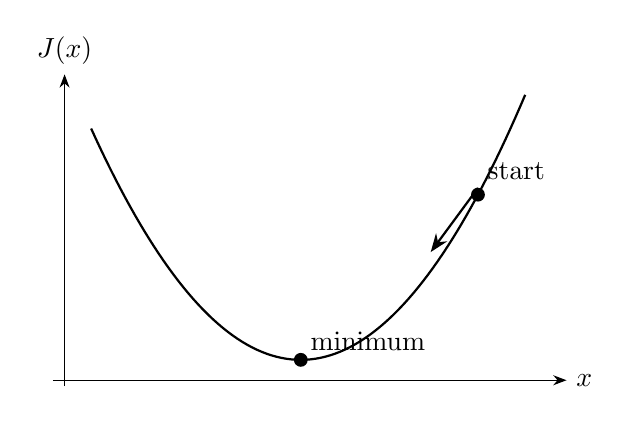
\begin{tikzpicture}[x=0.75cm,y=0.37cm,>=Stealth]
\draw[->] (-0.2,0)--(8.5,0) node[right] {$x$};
\draw[->] (0,-.2)--(0,10.5) node[above] {$J(x)$};
\draw[domain=0.45:7.8,samples=90,thick] plot (\x,{0.63*(\x-4)^2+0.7});
\fill (7,6.37) circle (2.5pt); \draw[->,thick] (7,6.6)--(6.2,4.4);
\fill (4,0.7) circle (2.5pt); \node[above right] at (4,0.7) {minimum};
\node[right] at (7,7.2) {start};
\end{tikzpicture}
\end{center}
\end{frame}

\begin{frame}{Why the negative derivative?}
For a small change $\Delta x$, a differentiable function obeys
\[
J(x+\Delta x)\approx J(x)+J'(x)\Delta x.
\]
Take $\Delta x=-\eta J'(x)$ with $\eta>0$:
\[
J(x+\Delta x)-J(x)\approx-\eta[J'(x)]^2\leq 0.
\]
\begin{itemize}
\item The derivative supplies the \emph{direction} and local steepness.
\item The learning rate $\eta$ controls the step size.
\item This predicts a decrease for sufficiently small steps; a large step can increase loss.
\end{itemize}
\end{frame}

\begin{frame}{The update rule}
\begin{center}
{\Large $\boxed{x_{t+1}=x_t-\eta J'(x_t)}$}
\end{center}
\vspace{0.4cm}
\begin{tabular}{ll}
$x_t$ & current location after $t$ updates\\[5pt]
$J'(x_t)$ & slope at the current location\\[5pt]
$\eta>0$ & learning rate (step-size multiplier)\\[5pt]
$x_{t+1}$ & updated location\\
\end{tabular}

\vspace{0.5cm}
For a parameter vector $\boldsymbol\theta$:
\[
\boxed{\boldsymbol\theta_{t+1}=\boldsymbol\theta_t-\eta\nabla J(\boldsymbol\theta_t)}.
\]
\end{frame}

\begin{frame}{Worked example 1: a parabola}
Consider the illustrative function also used in Nield's discussion:
\[
J(x)=(x-3)^2+4,\qquad J'(x)=2(x-3).
\]
Its minimum is $x^*=3$, with $J(x^*)=4$. Start at $x_0=0$ and choose $\eta=0.2$.
\[
x_{t+1}=x_t-0.2\cdot2(x_t-3)=0.6x_t+1.2.
\]
\begin{center}
\begin{tabular}{rrrr}
\toprule
$t$ & $x_t$ & $J'(x_t)$ & $J(x_t)$\\
\midrule
0 & 0.0000 & -6.0000 & 13.0000\\
1 & 1.2000 & -3.6000 & 7.2400\\
2 & 1.9200 & -2.1600 & 5.1664\\
3 & 2.3520 & -1.2960 & 4.4199\\
4 & 2.6112 & -0.7776 & 4.1512\\
\bottomrule
\end{tabular}
\end{center}
\end{frame}

\begin{frame}{What the example shows}
\begin{columns}[T]
\column{0.53\textwidth}
\begin{itemize}
\item The starting slope is $-6$; subtracting a negative quantity moves $x$ to the right.
\item As $x$ approaches 3, $|J'(x)|$ shrinks and steps become shorter.
\item The iterates approach 3, though a finite run may not reach it exactly.
\end{itemize}
\column{0.46\textwidth}
\begin{tikzpicture}[x=.76cm,y=.34cm,>=Stealth]
\draw[->] (0,0)--(5.4,0) node[right] {$x$};
\draw[->] (0,0)--(0,14) node[above] {$J$};
\draw[domain=0:5,samples=100,thick] plot (\x,{(\x-3)^2+4});
\foreach \x/\lab in {0/0,1.2/1,1.92/2,2.352/3,2.6112/4}{
\pgfmathsetmacro\yy{(\x-3)^2+4}
\fill (\x,\yy) circle (2.2pt);
}
\node[right] at (3,3.5) {$x^*=3$};
\end{tikzpicture}
\end{columns}
\end{frame}

\begin{frame}{Learning rate: too small, useful, too large}
For $J(x)=(x-3)^2+4$, let $e_t=x_t-3$.

Then
\[
e_{t+1}=(1-2\eta)e_t.
\]

\begin{center}
\begin{tabular}{lll}
\toprule
Learning rate & Error multiplier & Consequence\\
\midrule
$\eta=0.05$ & $0.90$ & converges slowly\\
$\eta=0.20$ & $0.60$ & converges smoothly\\
$\eta=0.75$ & $-0.50$ & oscillates but converges\\
$\eta=1.00$ & $-1.00$ & oscillates without convergence\\
$\eta=1.20$ & $-1.40$ & diverges\\
\bottomrule
\end{tabular}
\end{center}

For this particular quadratic, convergence from any starting $x_0$ occurs exactly when $0<\eta<1$.
\end{frame}

\begin{frame}{From one variable to many}
A regression line has two trainable parameters:
\[
\widehat y=mx+b,\qquad \boldsymbol\theta=\begin{bmatrix}m\\b\end{bmatrix}.
\]
The loss is a \emph{surface} over $(m,b)$, not a curve over $x$.
\[
\nabla J(m,b)=\begin{bmatrix}\partial J/\partial m\\[4pt]\partial J/\partial b\end{bmatrix}.
\]
Update both parameters simultaneously using gradients calculated at the same current point:
\[
\boxed{m_{t+1}=m_t-\eta\frac{\partial J}{\partial m}},\qquad
\boxed{b_{t+1}=b_t-\eta\frac{\partial J}{\partial b}}.
\]
\end{frame}

\begin{frame}{Choosing a regression loss}
Given observations $(x_i,y_i)$, let prediction errors be
\[
r_i=mx_i+b-y_i.
\]
We minimize the mean squared error with a convenient factor of $1/2$:
\[
\boxed{J(m,b)=\frac{1}{2n}\sum_{i=1}^n(mx_i+b-y_i)^2}.
\]
\begin{itemize}
\item Squaring makes both positive and negative errors costly.
\item Larger errors receive a larger penalty.
\item The factor $1/2$ cancels the $2$ introduced by differentiation.
\item This scaling has the same minimizer as ordinary sum of squared errors.
\end{itemize}
\end{frame}

\begin{frame}{Deriving the partial derivatives}
Use the chain rule for each squared residual:
\[
\frac{\partial}{\partial m}\frac{(mx_i+b-y_i)^2}{2n}
=\frac{1}{n}(mx_i+b-y_i)x_i.
\]
Similarly, the derivative with respect to $b$ multiplies by 1:
\[
\boxed{\frac{\partial J}{\partial m}=\frac1n\sum_{i=1}^n (mx_i+b-y_i)x_i}
\]
\[
\boxed{\frac{\partial J}{\partial b}=\frac1n\sum_{i=1}^n (mx_i+b-y_i)}.
\]
\smallskip
\alert{Interpretation:} the slope parameter reacts to error weighted by $x_i$; the intercept reacts to the average signed error.
\end{frame}

\begin{frame}{Worked example 2: fitting a line}
A deliberately small dataset allows every calculation to be checked by hand:
\[
(x_1,y_1)=(0,1),\qquad (x_2,y_2)=(1,3).
\]
Start with $m_0=0$, $b_0=0$, and $\eta=0.2$.
\begin{center}
\begin{tabular}{ccccc}
\toprule
$i$ & $x_i$ & $y_i$ & $\widehat y_i$ & $r_i$\\
\midrule
1 & 0 & 1 & 0 & $-1$\\
2 & 1 & 3 & 0 & $-3$\\
\bottomrule
\end{tabular}
\end{center}
\[
\frac{\partial J}{\partial m}=\frac{(-1)(0)+(-3)(1)}{2}=-1.5,
\qquad \frac{\partial J}{\partial b}=\frac{-1-3}{2}=-2.
\]
\end{frame}

\begin{frame}{First regression update: compute and check}
Gradient descent changes both parameters:
\[
m_1=0-0.2(-1.5)=0.3,\qquad b_1=0-0.2(-2)=0.4.
\]
The fitted prediction rule after one update is
\[\boxed{\widehat y=0.3x+0.4}.\]
Initial loss:
\[
J(0,0)=\tfrac14\big[(-1)^2+(-3)^2\big]=2.5.
\]
Updated loss:
\[
J(0.3,0.4)=\tfrac14\big[(-0.6)^2+(-2.3)^2\big]=1.4125.
\]
The loss decreases in one iteration. Continued updates approach the exact line $y=2x+1$.
\end{frame}

\begin{frame}{An executable Python implementation}
\small
\texttt{points = [(0.0, 1.0), (1.0, 3.0)]}\\
\texttt{m, b = 0.0, 0.0}\\
\texttt{eta = 0.2}\\[5pt]
\texttt{for step in range(200):}\\
\hspace*{1.4em}\texttt{n = len(points)}\\
\hspace*{1.4em}\texttt{dm = sum((m*x + b - y)*x for x, y in points)/n}\\
\hspace*{1.4em}\texttt{db = sum((m*x + b - y) for x, y in points)/n}\\
\hspace*{1.4em}\texttt{m -= eta*dm}\\
\hspace*{1.4em}\texttt{b -= eta*db}\\[7pt]
\texttt{print(m, b)  \# close to (2, 1)}
\vspace{0.5cm}
\begin{itemize}
\item Compute \texttt{dm} and \texttt{db} \emph{before} updating either parameter.
\item The chosen learning rate works for this illustrative dataset, not necessarily for arbitrary datasets.
\end{itemize}
\end{frame}

\begin{frame}{Batch versus stochastic gradient descent}
\begin{tabular}{p{0.23\textwidth}p{0.33\textwidth}p{0.33\textwidth}}
\toprule
 & Full-batch GD & Stochastic GD (SGD)\\
\midrule
Gradient uses & Every training example & One randomly selected example\\[5pt]
Updates & One per full pass & Many within each pass\\[5pt]
Trajectory & Relatively smooth & Noisier\\[5pt]
Typical benefit & Stable gradient estimate & Lower cost per update; useful at scale\\
\bottomrule
\end{tabular}
\vspace{0.5cm}
\begin{itemize}
\item \textbf{Mini-batch GD} uses a small set of examples per update.
\item With SGD, a decaying learning rate can help reduce fluctuation near a minimum.
\end{itemize}
\end{frame}

\begin{frame}{When does gradient descent stop?}
Practical stopping criteria include:
\begin{itemize}
\item Gradient magnitude becomes small: $\|\nabla J(\boldsymbol\theta_t)\|<\varepsilon$.
\item Improvement in loss becomes negligible.
\item A preset iteration or compute budget is reached.
\item Validation error stops improving (important in predictive modeling).
\end{itemize}
\vspace{0.2cm}
\textbf{Cautions:} A zero gradient may indicate a minimum, maximum, or saddle point; nonconvex losses may have multiple local minima. Feature scaling may improve optimization behavior.
\end{frame}

\begin{frame}{Classroom check: calculate the next step}
Let $J(x)=(x-3)^2+4$, with $x_0=5$ and $\eta=0.25$.
\begin{enumerate}
\item What is the derivative at $x_0$?
\item What is $x_1$?
\item Compare $J(x_0)$ and $J(x_1)$.
\end{enumerate}
\vspace{0.5cm}
\textbf{Solution:}\quad $J'(5)=4$,\quad $x_1=5-0.25(4)=4$,\quad $J(5)=8$,\quad $J(4)=5$.
\end{frame}

\begin{frame}{Key takeaways}
\begin{enumerate}
\item A derivative (or gradient) identifies the direction of steepest local increase.
\item Subtracting a scaled gradient moves toward lower loss when the step is sufficiently small.
\item Learning rate determines how quickly and reliably the method progresses.
\item Linear regression uses the same logic to update slope and intercept.
\item Iterative optimization generalizes far beyond simple regression.
\end{enumerate}
\end{frame}
\end{document}
